\documentclass[12pt]{article}
\usepackage{verbatim}
\usepackage[dvips]{epsfig}
\usepackage{color}
\usepackage{url}
\usepackage[colorlinks=true]{hyperref}

\begin{document}

\section*{GENESIS: Documentation}

{\bf Related Documentation:}
% start: userdocs-tag-replace-items related-do-nothing
% end: userdocs-tag-replace-items related-do-nothing

\section*{Publication Review}

Current reviews of modeling papers are based entirely on reading text. In contrast the review process we propose will actually start with a first phase of automated model validation.  This validation process will be exercised by the author themselves and provide feedback to the author on possible concerns regarding their model.  This facility will allow the author to either correct, or specifically provide arguments as to why the model is worthy of publication anyway.  In effect this system will therefore iteratively develop a set of accepted basic standards for model publication, while providing an opportunity to argue for the extension or replacement of those standards.  Once this level of automated review is passed, the model will be made available to reviewers, who can evaluate the authors arguments with respect to core features of the model, and then consider the additional capabilities of the model as demonstrated by the figures and their annotation.  It is important to note that the modular nature of the core infrastructure for this project will allow us to take advantage of other approaches to model evaluation\,\cite{Cannon:2006pi}. The proposed process is illustrated in the following figure:  

\begin{figure}[h]
  \centering
   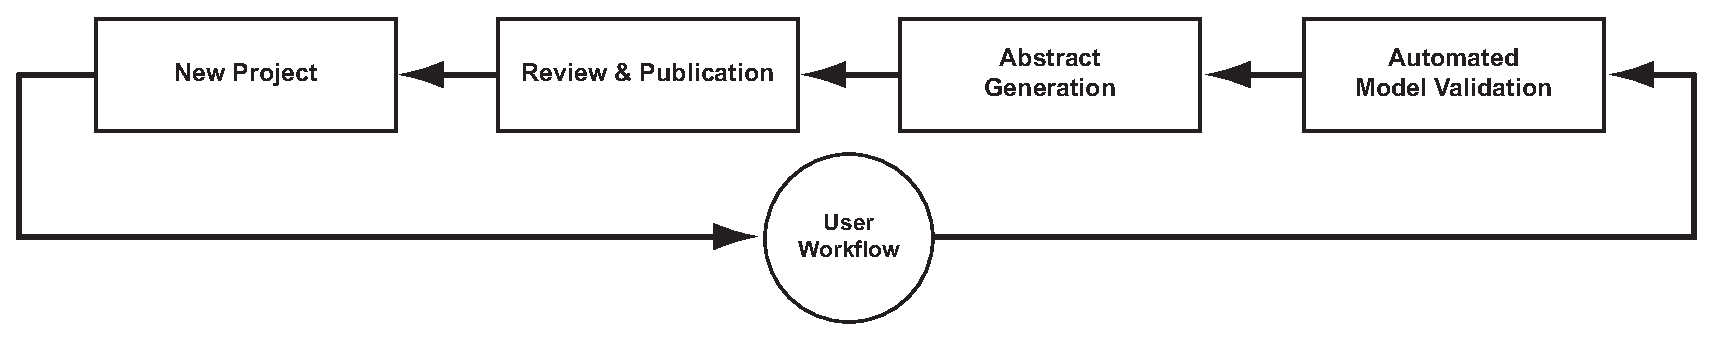
\includegraphics[scale=0.5]{figures/publication-workflow.eps}
%\caption{{\bf A Dummy Figure:} Example of \LaTeX\,\,\,code to incorporate a figure into documentation.}
  \label{fig:pub-wflow}
\end{figure}

\begin{enumerate}
   \item  {\bf Verify model:} This step in the Publication-Workflow is to ensure that the lineage starting point of the model employed for simulations is a previously published source model. Model verification is performed on the morphology, cable discretization, equations for different membrane and synaptic channel types and their kinetics, model parameter values, and dynamic response to specific current injection and voltage clamp protocols.
   \item  {\bf  Validate model:} In the absence of a pre-existing model, model validation is completed by the generation of tables and figures reporting model verification. These data are acquired from the Model-Container. If the model is based on a pre-existing published model, validation is completed by a comparison of the two models. Any differences between the two models are identified, characterized, quantified, and reported. This step can be performed by a user prior to submission to a publication data base.
   \item  {\bf Parameter Space:} The issue of parameter space analysis is important and complex and still very much an area of open research, especially for complex models\,\cite{Baldi:1998qa, vanier99:_compar_survey_autom_param_searc}. However, there are mechanisms available to examine the sensitivity of core modeling results to parameter variations\,\cite{Achard:2006mb}.  We anticipate that a model publication system is likely to accelerate the development of this aspect of model analysis and validation.
\end{enumerate}

\subsection*{Implementation Details}

Space does not allow a full description of the implementation details.  However, there are a few key components to the system that are now briefly described:

\begin{enumerate}
   \item {\bf Database Format:} Each database supports system-specific, project-specific, and user-specific views. The system view abstracts system specific configurations such as the filesystem layout. The project view is a container for project specific data such as models and source code. The user view gives the user the flexibility to run simulations without initiating a new research project. The existing GENESIS repositories implement these views based on system process environment settings.

The database structure has three major features: (i) It complements the steps of the \href{../workflow-user/workflow-user.tex}{\bf User\,Workflow}, (ii) It provides a database of text, figures, and annotations, and (iii) Defines relationships between other objects in the database. 

Based on the existing Documentation System each database described below will initially be implemented as a YAML-tagged flat file system. This approach, also in use by popular databases in neuroscience (eg. www.neuromorpho.org) allows convenient storage of the highly heterogeneous data typical of neuroscience models using specially formatted text based files. Other advantages include easy manipulation, archiving, and synchronization between databases using the file distribution technology and replication technology developed for the {\bf Project\,Browser}.

The databases that will be developed to support the Publication-Workflow complement the databases of the User-Workflow:
\begin{enumerate}
\item {\bf Publication Narrative Component Repository:} The database with the narrative components of a publication serves two purposes: the definition of collections of fragments of simulation configurations allows traditional-style publication figures to be reproduced. Secondly, inserting free-style text paragraphs and combining them with the figures allows for profound discussion sections. Also personal notes, reviewer comments, and computer generated annotations can be inserted.
\item {\bf Publication Object Relationships Repository:} The relationships between all the objects of a model publication are defined in this database. As an example, the main menu of a publication is defined as a narrative component, and is linked to its contents via a set of records in this database. Not only does this allow customization of the main menu to the contents of a model publication, but it also provides for the definition of secondary reader-flows through one or more publications. The implementation will be based on the YAML tags that were developed for the Documentation System. For a typical model publication we envisage that at least the following flows will be defined: 'history', outlining the history of the model, 'present', giving an overview of related models, and 'tutorial', tutorializing the functions implemented by the published model. In addition to these narrative flows, we will also define flows that are specific to verification, validation, and review. As an example, every single-cell model should come with an automatically generated report that guarantees model parameters are within their physiological range. The publication system described here greatly expands the current limitations of paper publication that are bound by a predefined and linear flow.
\item {\bf Database Tools:} We plan to develop additional interfaces for the sole purpose of examining, exploring, querying, and comparing the models in the database, including their micro- and macro-evolution.  For example we will develop tools that visualize the channel distribution over a morphology and compare the different implementations of a specific channel type.  As an extension of the automated benchmark test suite other software under development includes robots that validate the static structure of the models in the database, including parameter range testers, morphological constraint testers and robots that check for shared features in a model. Server side based, this framework needs further extension before it also becomes useful to researchers. We also plan to develop robots that detect database model similarities and propose actions to the user.
\item {\bf Database Distribution and Replication Strategies:} The Project-Browser distributes the data of a single research project over multiple computers. After creation of data on any one computer the {\bf Project\,Browser} distribution policy replicates parts of the project database on different computers as required using a secure shell as a transport mechanism. The same data distribution mechanism also facilitates collaborations between labs that trust one another.  Research projects typically proceed by incrementally gathering result data from simulations, so we plan to evaluate other policies that provide explicit support for incremental distribution of data, such as the {\it rsync} protocol.
\end{enumerate}
Electronic publication submission replicates the research project database at the publisher's hardware infrastructure. Both automated and manual review processes generate new data that is stored in the database. These data can then be compiled into a review report that becomes an integral part of the electronic publication.

Accepted electronic publications can be replicated at a local computer of a reader using the same distribution policies. By default the most important components of a research project will be replicated, but options will be available to replicate all data in the research project, including meta-data that was produced during the review.
\item {\bf Integrity, Access Control and DRM:} Digital rights management (DRM, also sometimes called Information Rights Management) is a generic term for access control to a database to protect confidential content. DRM will be implemented using cryptographic key pairs and checksums.  Each account in the publication system will generate a public and private key. The private key is stored on a user computer and is one half of user identification, while the public key completes user identification and can be duplicated and stored on many computers.  Public/private key pairs can also belong to 'machine' accounts, for example for robot based automated model verification. To protect the system from unauthorized access and to preserve data integrity cryptographic checksums on the content of the files in the database are compared to authenticate both queries and data. Optionally, these checksums can then be signed using an account's private key. 

Computing and comparing the cryptographic checksums after pulling data from an external database guarantees the origin and integrity of the pulled annotations, including reviewer comments and computer validation test results. This implementation guarantees the scientific quality of  a model that is considered for starting a research project. The result will be an infrastructure to maintain a distributed database of computational neuroscience models, their annotations, and narrative flows.

The DRM system designed for the publication system will integrate the distributed nature of a research project database and the different roles a user can have when reading and modifying an electronic publication. The design is similar to that of well-known service-driven websites such as Facebook (www.facebook.com) and Blogger (www.blogger.com).
\end{enumerate}

\subsection*{Adoption of the Publication System}

It is possible that investigators might raise objections to adopting the publication system outlined in this proposal particularly with regard to licensing and copyright. There are two recognized blocks to truly reproducible research (a fundamental purpose of both the scientific method and any comprehensive electronic publication system): firstly the lack of reward for producing reproducible work and secondly the legal obstacles to the full sharing of methods, code, data, figures and publication\,\cite{Stodden:2009cq}. The first objection is overcome through the provision of lineage tracking and attribution by the proposed publication system. To resolve the second block we will evaluate a number of alternative licensing and copyright procedures, one of which is the Reproducible Research Standard (RSS).  This provides a legal basis to encourage replicable scientific investigation through attribution, the facilitation of greater collaboration, and the promotion of the engagement of the larger community in scientific learning and discovery\,\cite{Stodden:2009cq}. In brief, RRS is a compilation of other licenses by treating individual compendium elements of a scientific publication separately. It can be used to rescind the aspects of copyright that prevent scientists from sharing important research information.  It eliminates the viral license proliferation inherent in the domain of computational based research when using other licenses such as the GPL and BSD.

\bibliographystyle{plain}
\bibliography{../tex/bib/g3-refs}

\end{document}
